\section{実験結果と考察}

\subsection{α相試料への変換}

α相からβ相への相転移にかかる時間は、形状や表面性状に強く依存する。\cite{Matvienko}
特に、筆者は相転移の核生成がの端で起こりやすく、であることを確かめた。
表\ref{tab:trans_Time}に、相転移にかかったデータをまとめる。

Matvienkoらの研究\cite{Matvienko}によると、βスズ中に分散したGe相転移は相転移速度を遅くするため、試料1の相転移が非常に遅いことが理解できる。

\begin{table}[htb]
    \begin{center}
  \begin{tabular}{c|cccc}
    & 試料1(Ge1\%/急冷) & 試料2(Ge0.5\%/急冷) & 試料3(Ge0.1\%/急冷)& 試料6(Ge1\%/急冷) \\ \hline
    As grown & 1ヶ月以上 & 一週間以内 & 一週間以内 & 数日 \\
    表面に傷をつける & 3ヶ月以内 & && \\
    Ge核押し付け& 3ヶ月以内 & & &  \\
  \end{tabular}
  \caption{β相からα相への転移にかかる時間}
  \label{tab:trans_Time}
    \end{center}
\end{table}


\subsection{試料のX線回折}
まず(as grown)試料に関して、述べる。


アモルファス構造を持つ石英ガラスのハロー回折であると筆者は考える。しかしこのブロードなスペクトルの影響は無視できる。

\begin{figure}[htb]
    \begin{center}
   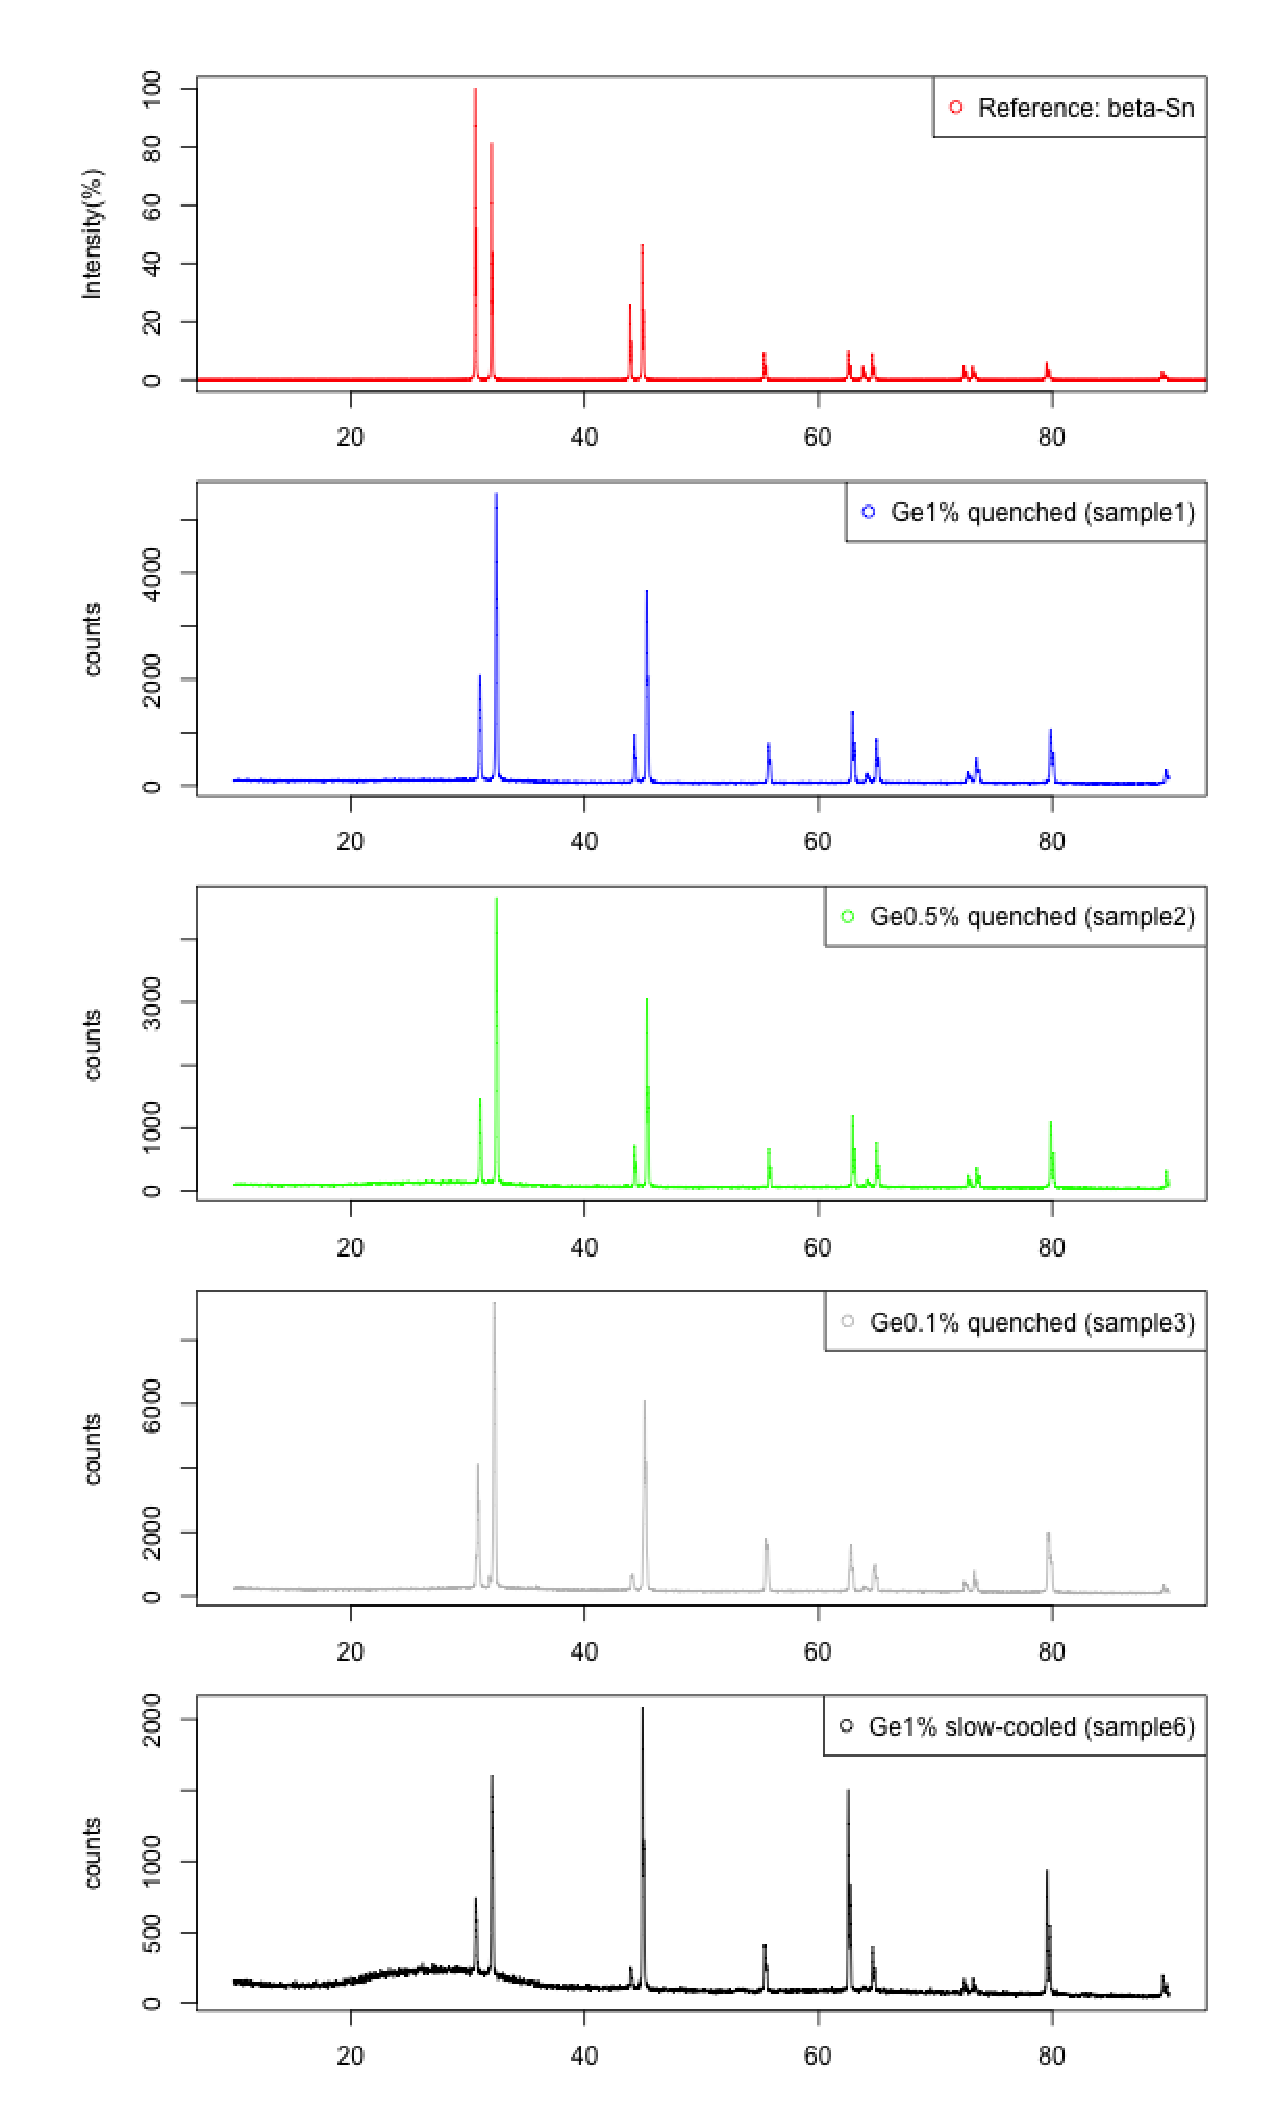
\includegraphics[width=150mm]{results_discussions/intensity_asgrown_samples.eps}
  \end{center}
  \caption{As grown(β相)試料}
  \label{fig:intensity_pested_samples}
\end{figure}

\begin{figure}[htb]
    \begin{center}
   \includegraphics[width=150mm]{results_discussions/intensity_pested_samples.eps}
  \end{center}
  \caption{α相に変換された試料}
  \label{fig:intensity_pested_samples}
\end{figure}
%\subsection{スズ-Ge合金試料(β相とα相)のEdX}

\subsection{α相からβ相への転移温度}
作成後、家庭用冷蔵庫の冷凍室に保持しα相に変換した試料に関して、加熱しながら抵抗測定を行ったところ、ある温度以上で抵抗が大きく落ち込んだ。半導体のα相から金属のβ相への相転移であると筆者は考える。

表\ref{tab:transT}に見積もった相転移温度を示す。
\begin{table}[htb]
  \begin{center}
  \begin{tabular}{cccc}
    試料1(Ge1\%/急冷) & 試料2(Ge0.5\%/急冷) & 試料3(Ge0.1\%/急冷)& 試料6(Ge1\%/徐冷) \\ \hline
    NN & $364\pm3$ & $337.5\pm1$ & $347\pm4$ \\
     &                & $338.5\pm2$ &                \\
  \end{tabular}
  \caption{α相からβ相への転移温度}
  \label{tab:transT}
    \end{center}
\end{table}

\begin{table}[htb]
    \begin{center}
  \begin{tabular}{ccc}
    Ge1\%/急冷 & Ge0.5\%/急冷 & Ge0.1\%/急冷  \\ \hline
    $328.3\pm0.3$ & $346.6\pm4.0$ & $354.2\pm0.1$ \\
  \end{tabular}
  \caption{α相からβ相への転移温度(先行研究\cite{})}
  \label{tab:transT_ref}
    \end{center}
\end{table}

\begin{figure}[htb]
    \begin{center}
   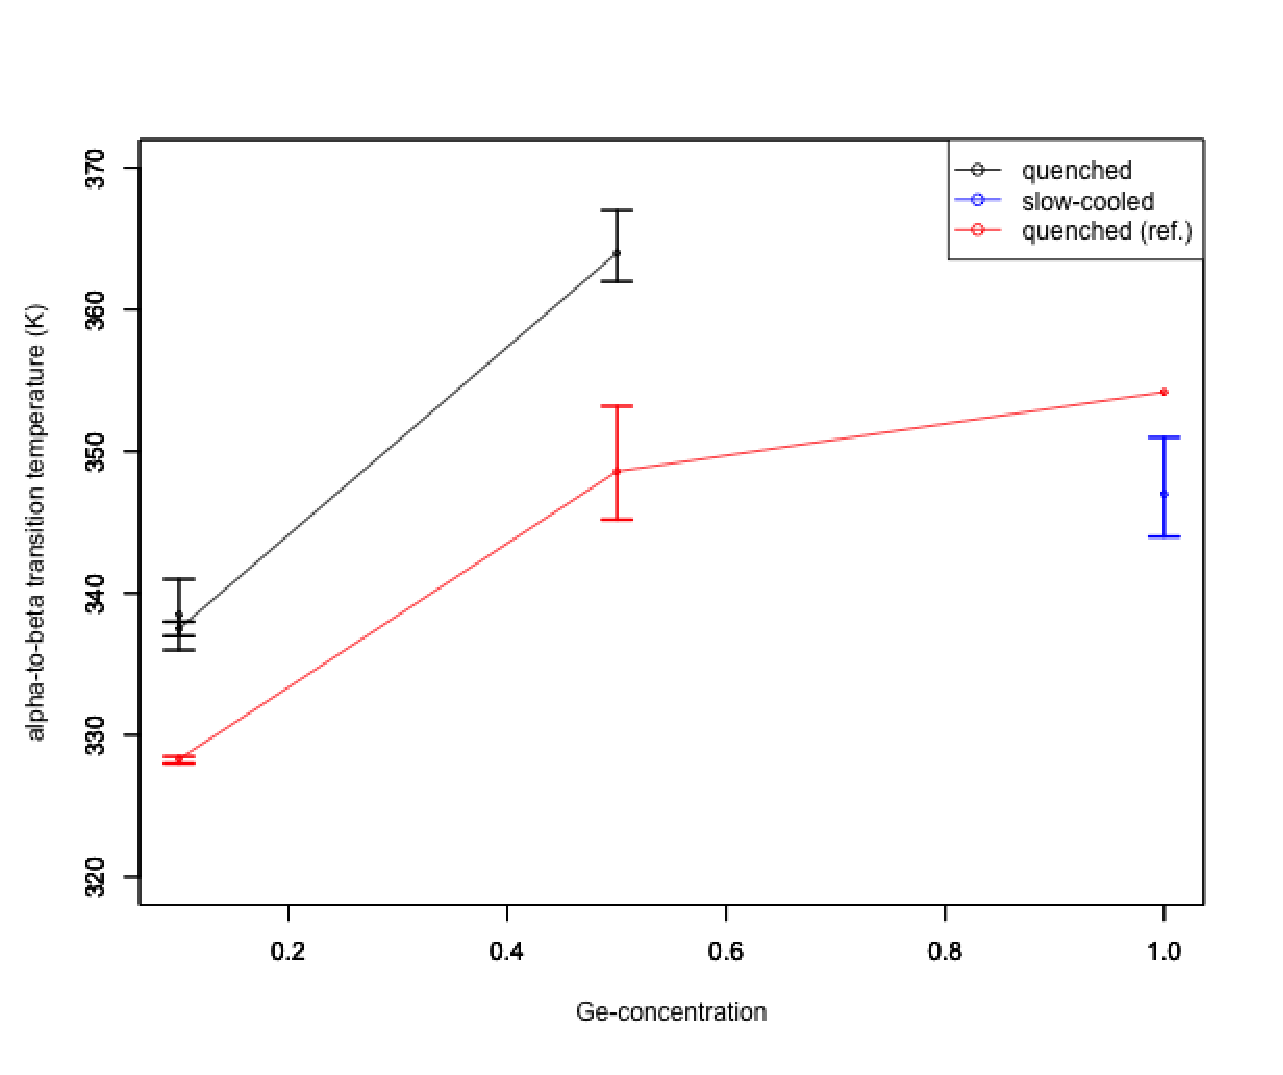
\includegraphics[width=130mm]{results_discussions/TransitionT.eps}
  \end{center}
  \caption{α相からβ相への転移温度}
  \label{fig:TransitionT}
\end{figure}

\subsection{電流パルスを用いたα相からβ相への変換}
図\ref{fig:181228_before_after_pulse_log}に電流パルス印加前後の抵抗値を示す。パルス印加前(赤色)の抵抗は温度を小さくしながら測定したもので、温度が小さくなるほど抵抗が小さく、半導体的な温度-抵抗依存性を示す。

一方、パルス印加後の抵抗(青色)は60Kより低温で温度が小さくなっていることがわかる。この領域で金属からの寄与が大きく、超伝導体転移が確認できた。

では金属との並列として理解できる\cite{Mayr,McLachlan}

\begin{figure}[htb]
    \begin{center}
   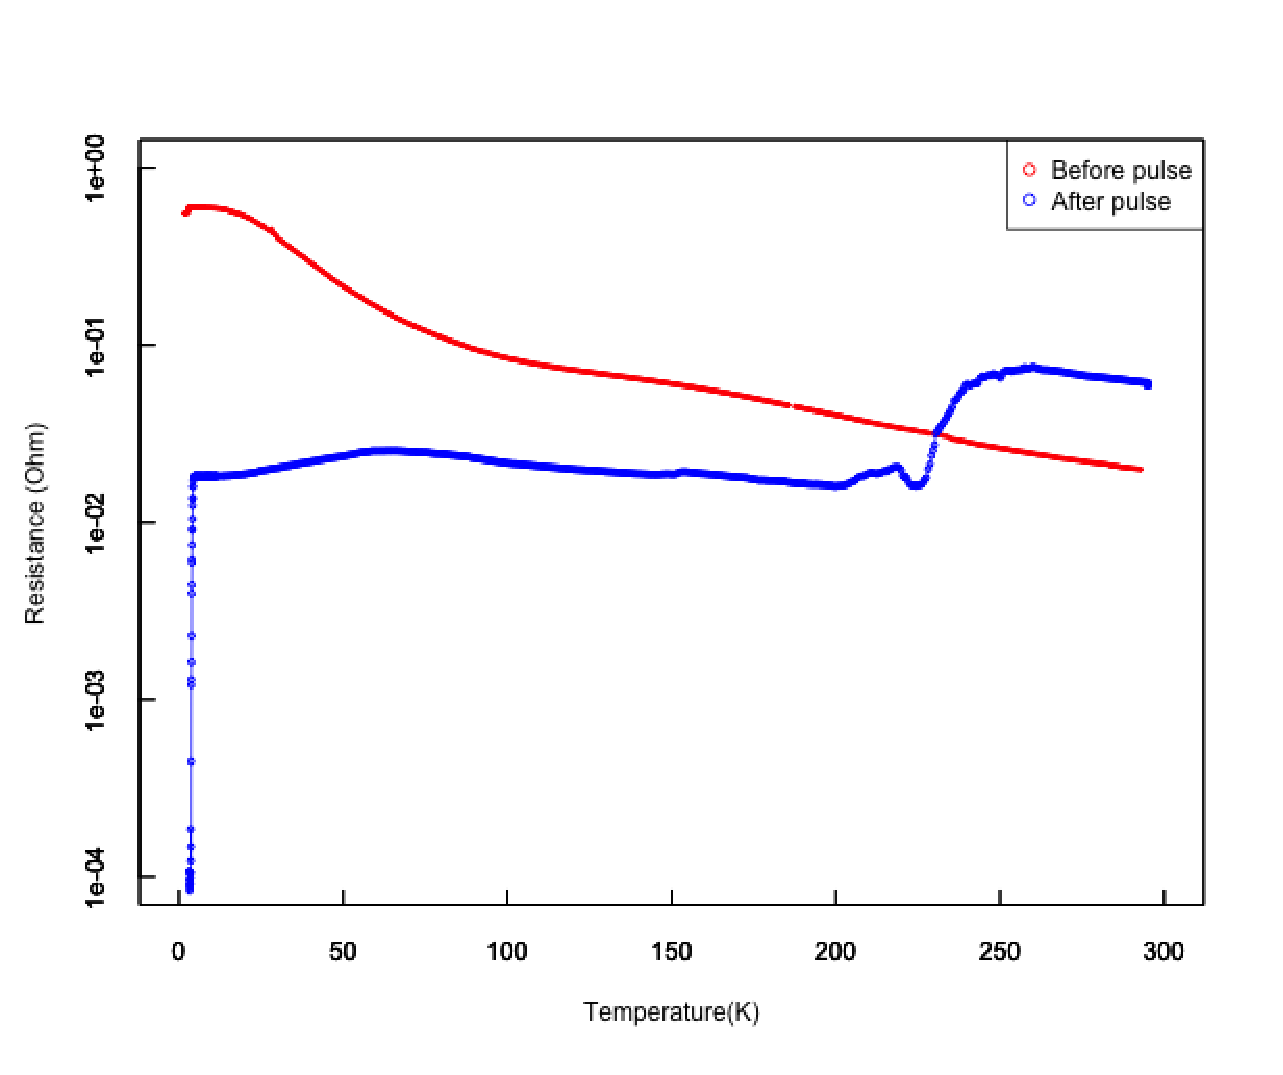
\includegraphics[width=150mm]{results_discussions/181228_before_after_pulse_log.eps}
  \end{center}
  \caption{}
  \label{fig:181228_before_after_pulse_log}
\end{figure}

\begin{figure}[htb]
 \begin{minipage}{0.5\hsize}
    \begin{center}
   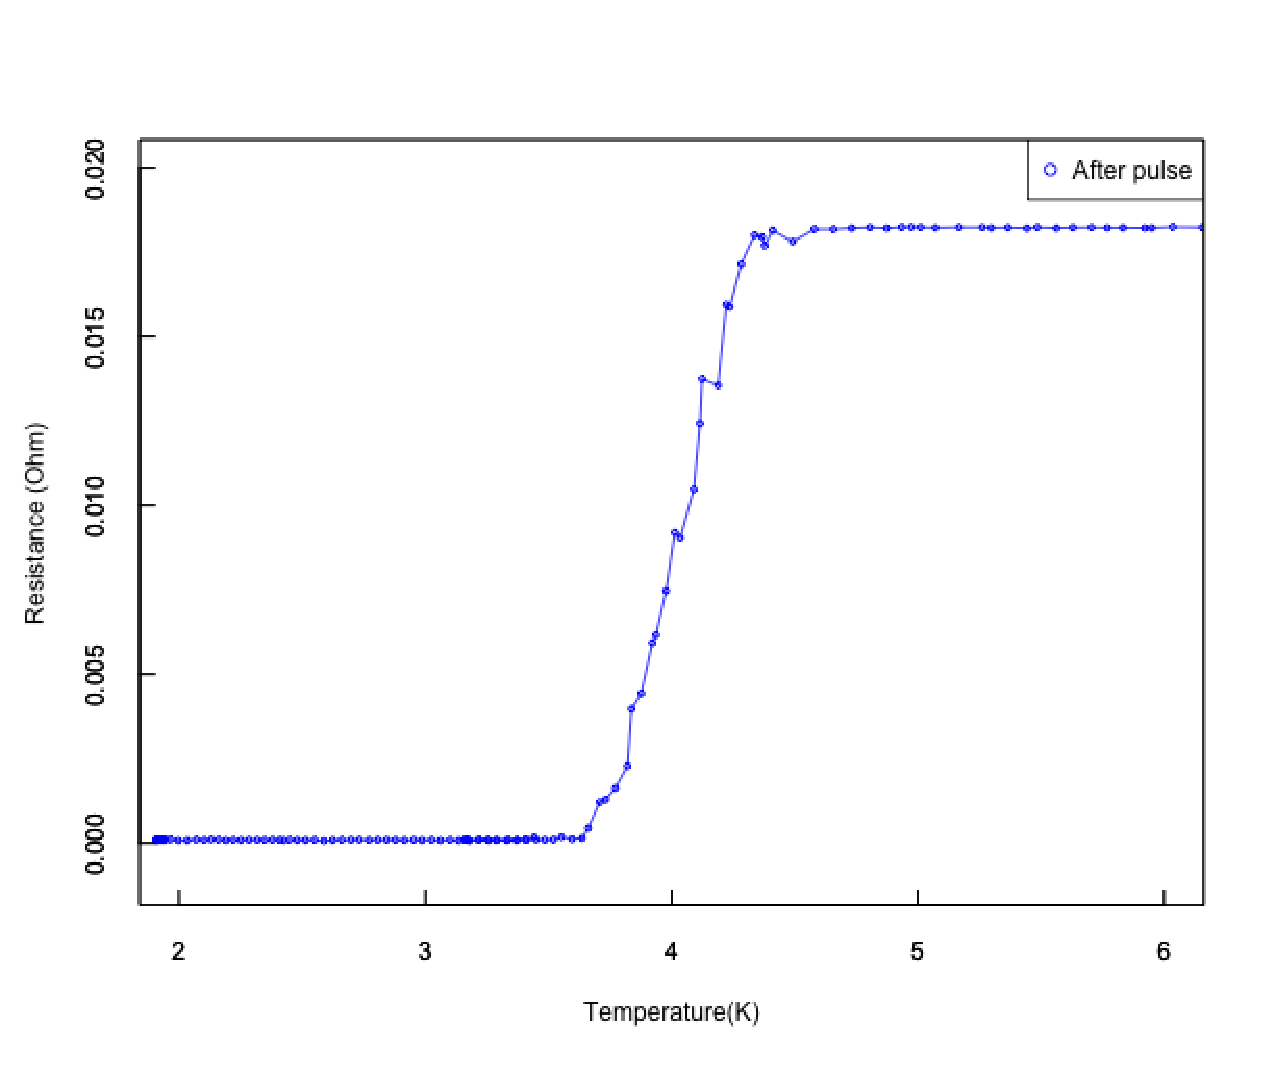
\includegraphics[width=\hsize]{results_discussions/181228_after_pulse.eps}
  \end{center}
  \caption{}
  \label{fig:181228_after_pulse}
 \end{minipage}
 \begin{minipage}{0.5\hsize}
     \begin{center}
   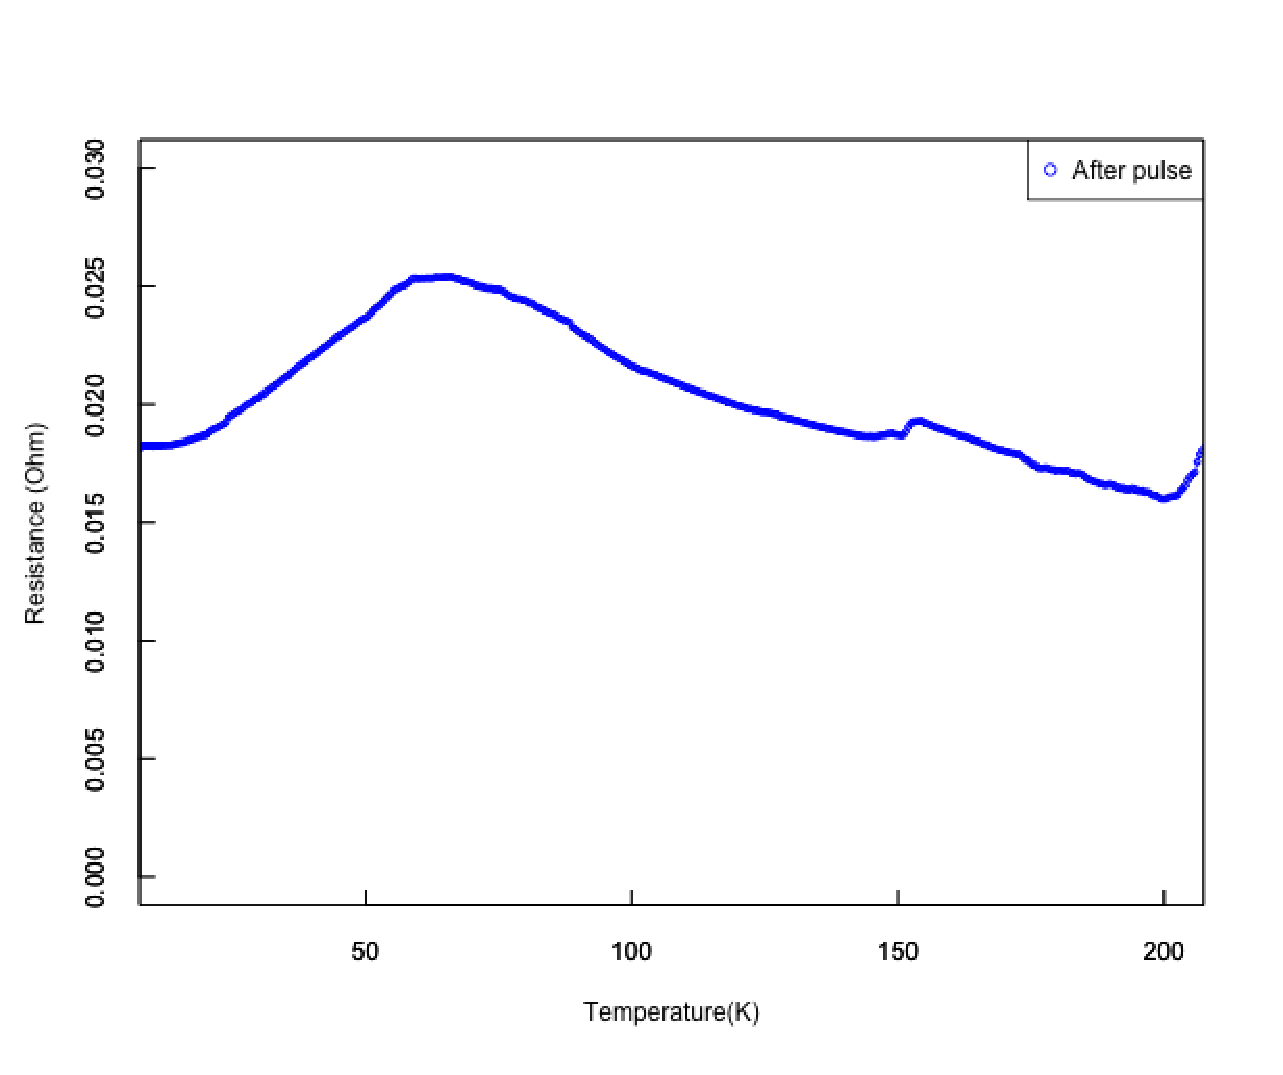
\includegraphics[width=\hsize]{results_discussions/181228_after_pulse2.eps}
  \end{center}
  \caption{}
  \label{fig:181228_after_pulse2}
   \end{minipage}
\end{figure}


\begin{figure}[htb]
 \begin{minipage}{0.5\hsize}
    \begin{center}
   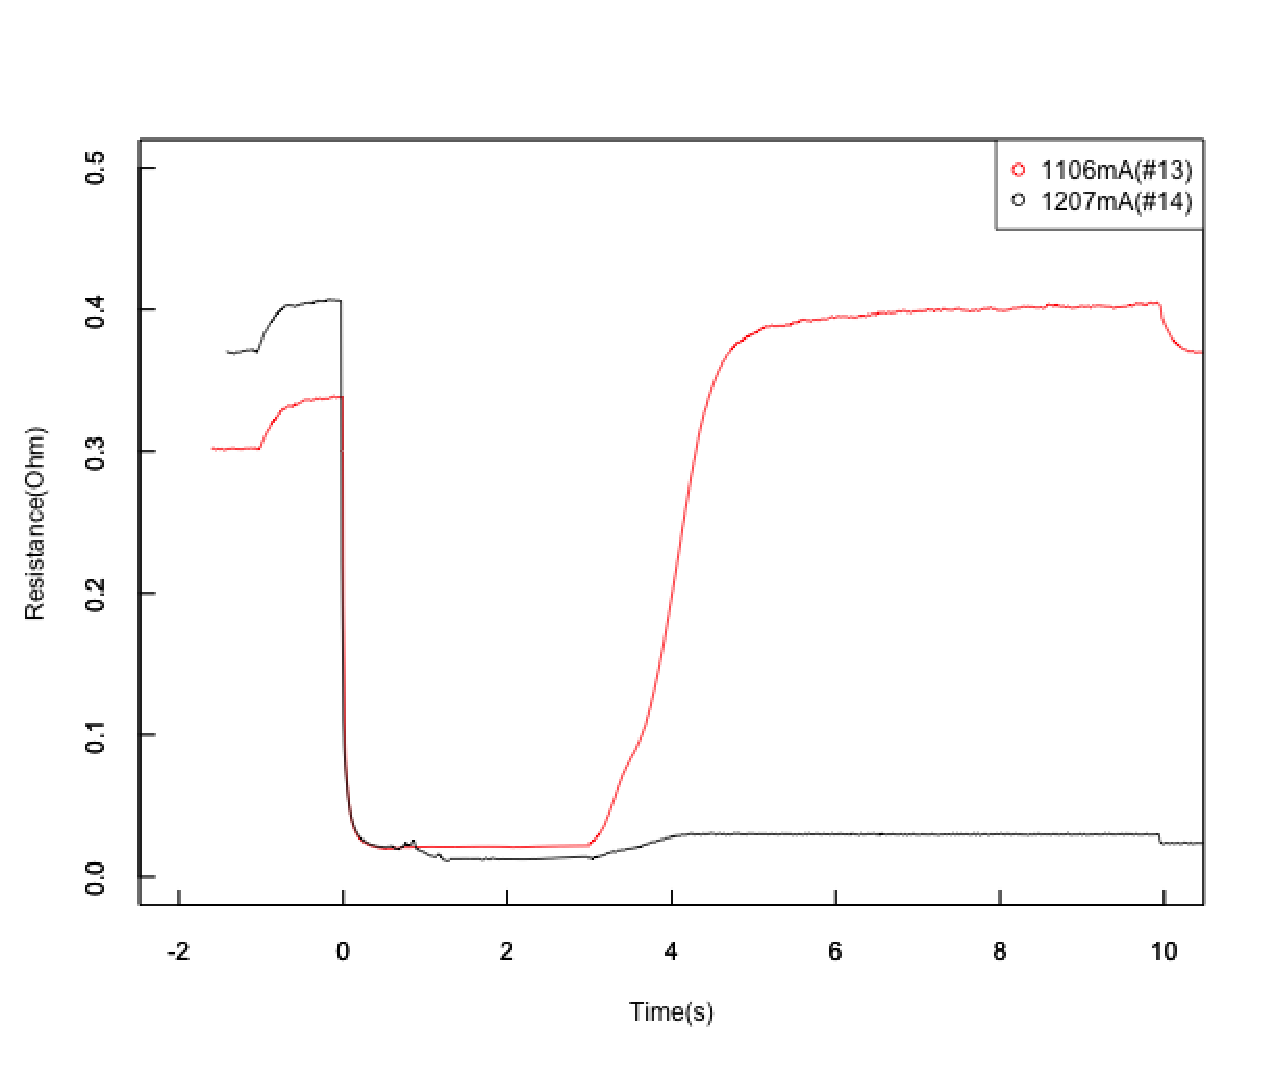
\includegraphics[width=\hsize]{results_discussions/181228_Resistance_pulse_selected.eps}
  \end{center}
  \caption{}
  \label{fig:181228_Resistance_pulse_selected}
 \end{minipage}
 \begin{minipage}{0.5\hsize}
     \begin{center}
   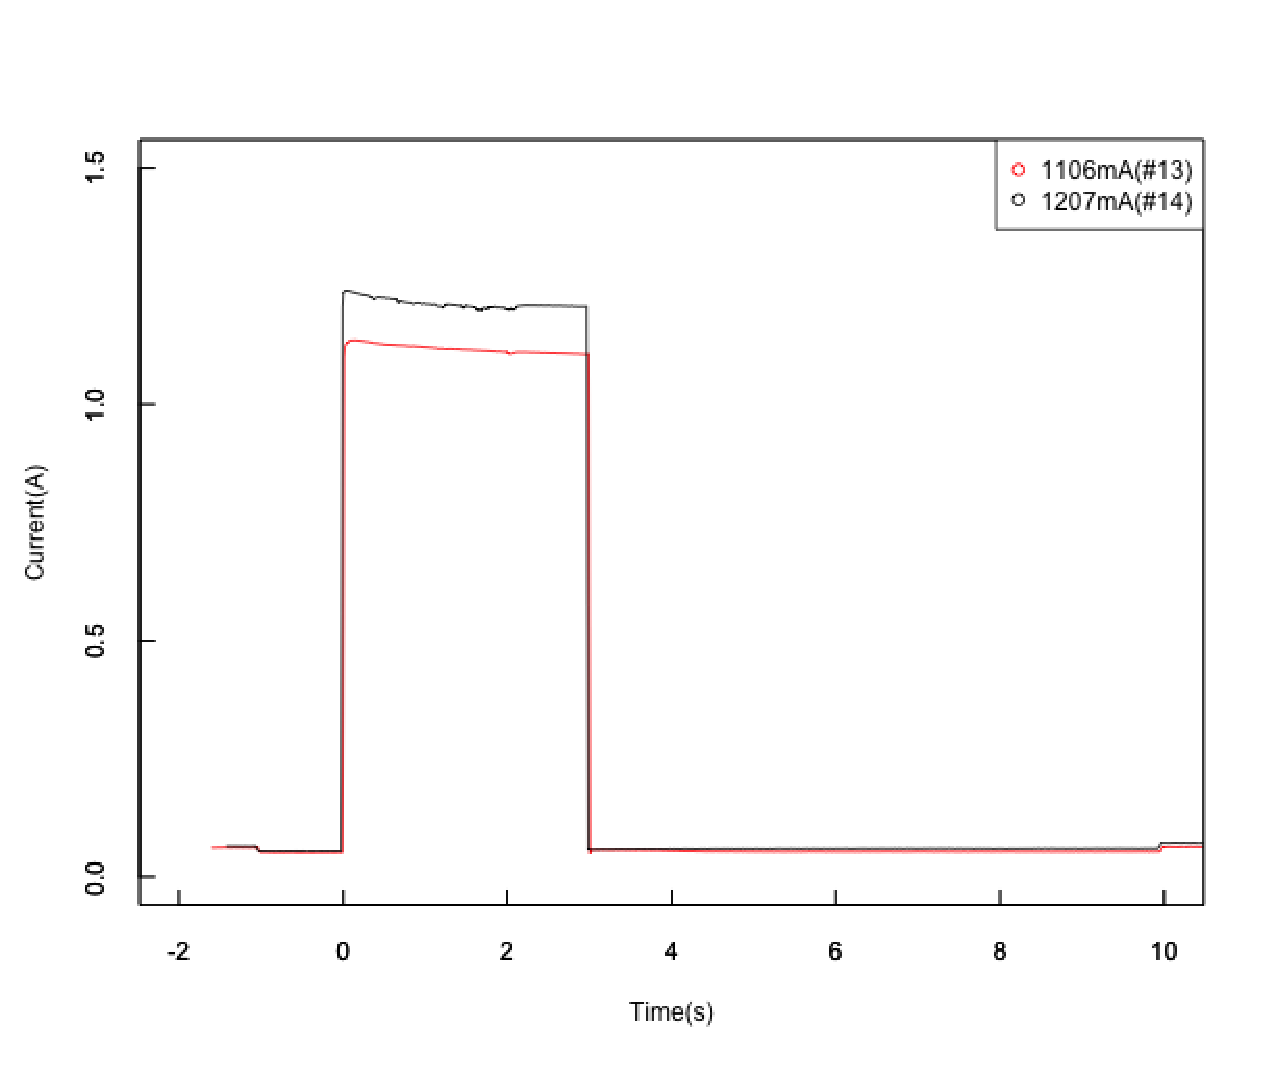
\includegraphics[width=\hsize]{results_discussions/181228_current_pulse_selected.eps}
  \end{center}
  \caption{}
  \label{fig:181228_current_pulse_selected}
   \end{minipage}
\end{figure}


\subsection{電流パルスによるα相とβ相の共存状態の生成}
\begin{figure}[htb]
 \begin{minipage}{0.5\hsize}
    \begin{center}
   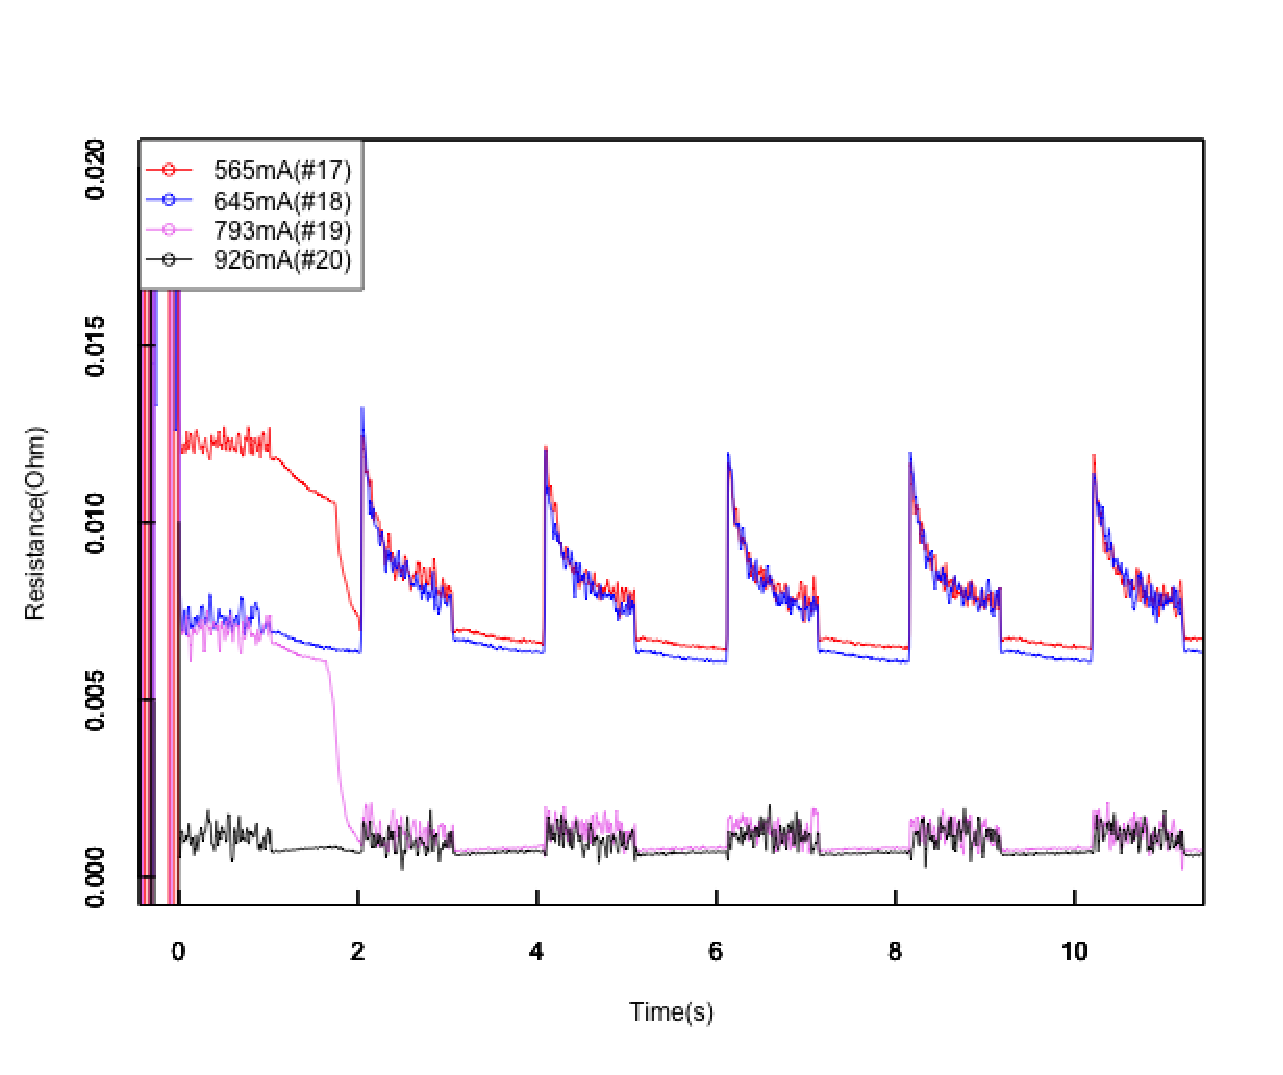
\includegraphics[width=\hsize]{results_discussions/190112_Resistance_pulse.eps}
  \end{center}
  \caption{}
  \label{fig:190112_Resistance_pulse}
 \end{minipage}
 \begin{minipage}{0.5\hsize}
     \begin{center}
   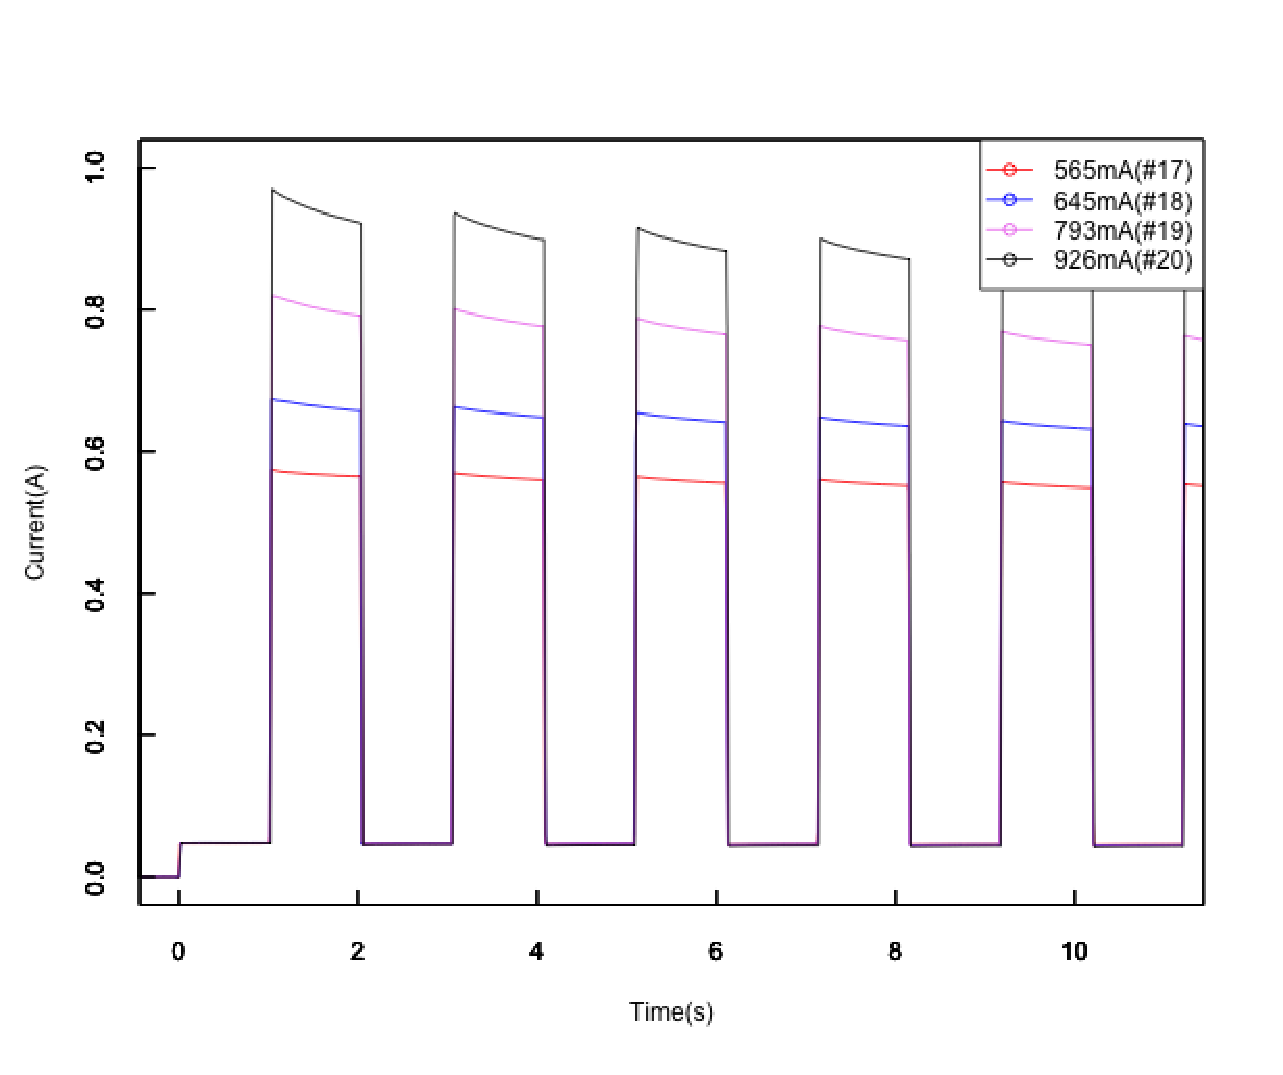
\includegraphics[width=\hsize]{results_discussions/190112_Current_pulse.eps}
  \end{center}
  \caption{}
  \label{fig:190112_Current_pulse}
   \end{minipage}
\end{figure}

\begin{figure}[htbp]
 \begin{minipage}{0.5\hsize}
  \begin{center}
   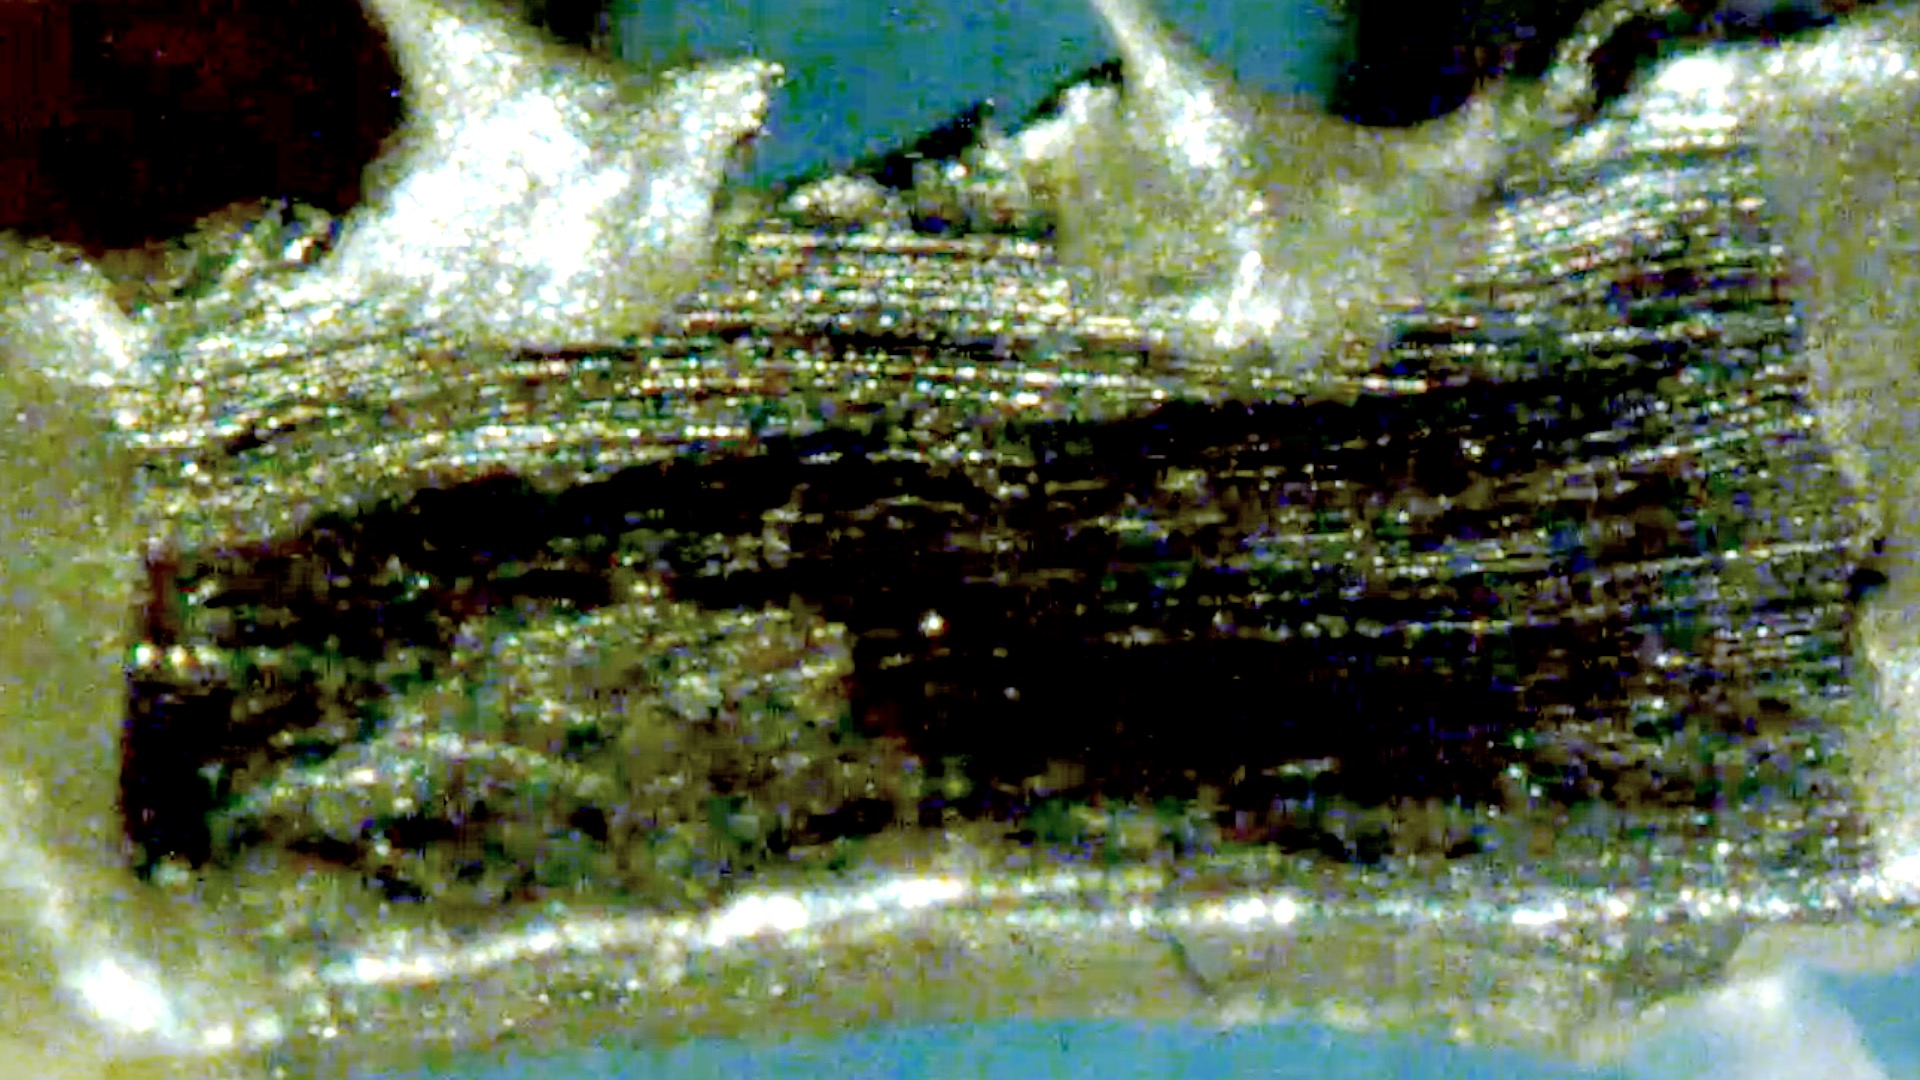
\includegraphics[width=\hsize]{results_discussions/190112_before_pulse17.eps}
  \end{center}
  \caption{}
  \label{fig:one}
 \end{minipage}
 \begin{minipage}{0.5\hsize}
  \begin{center}
   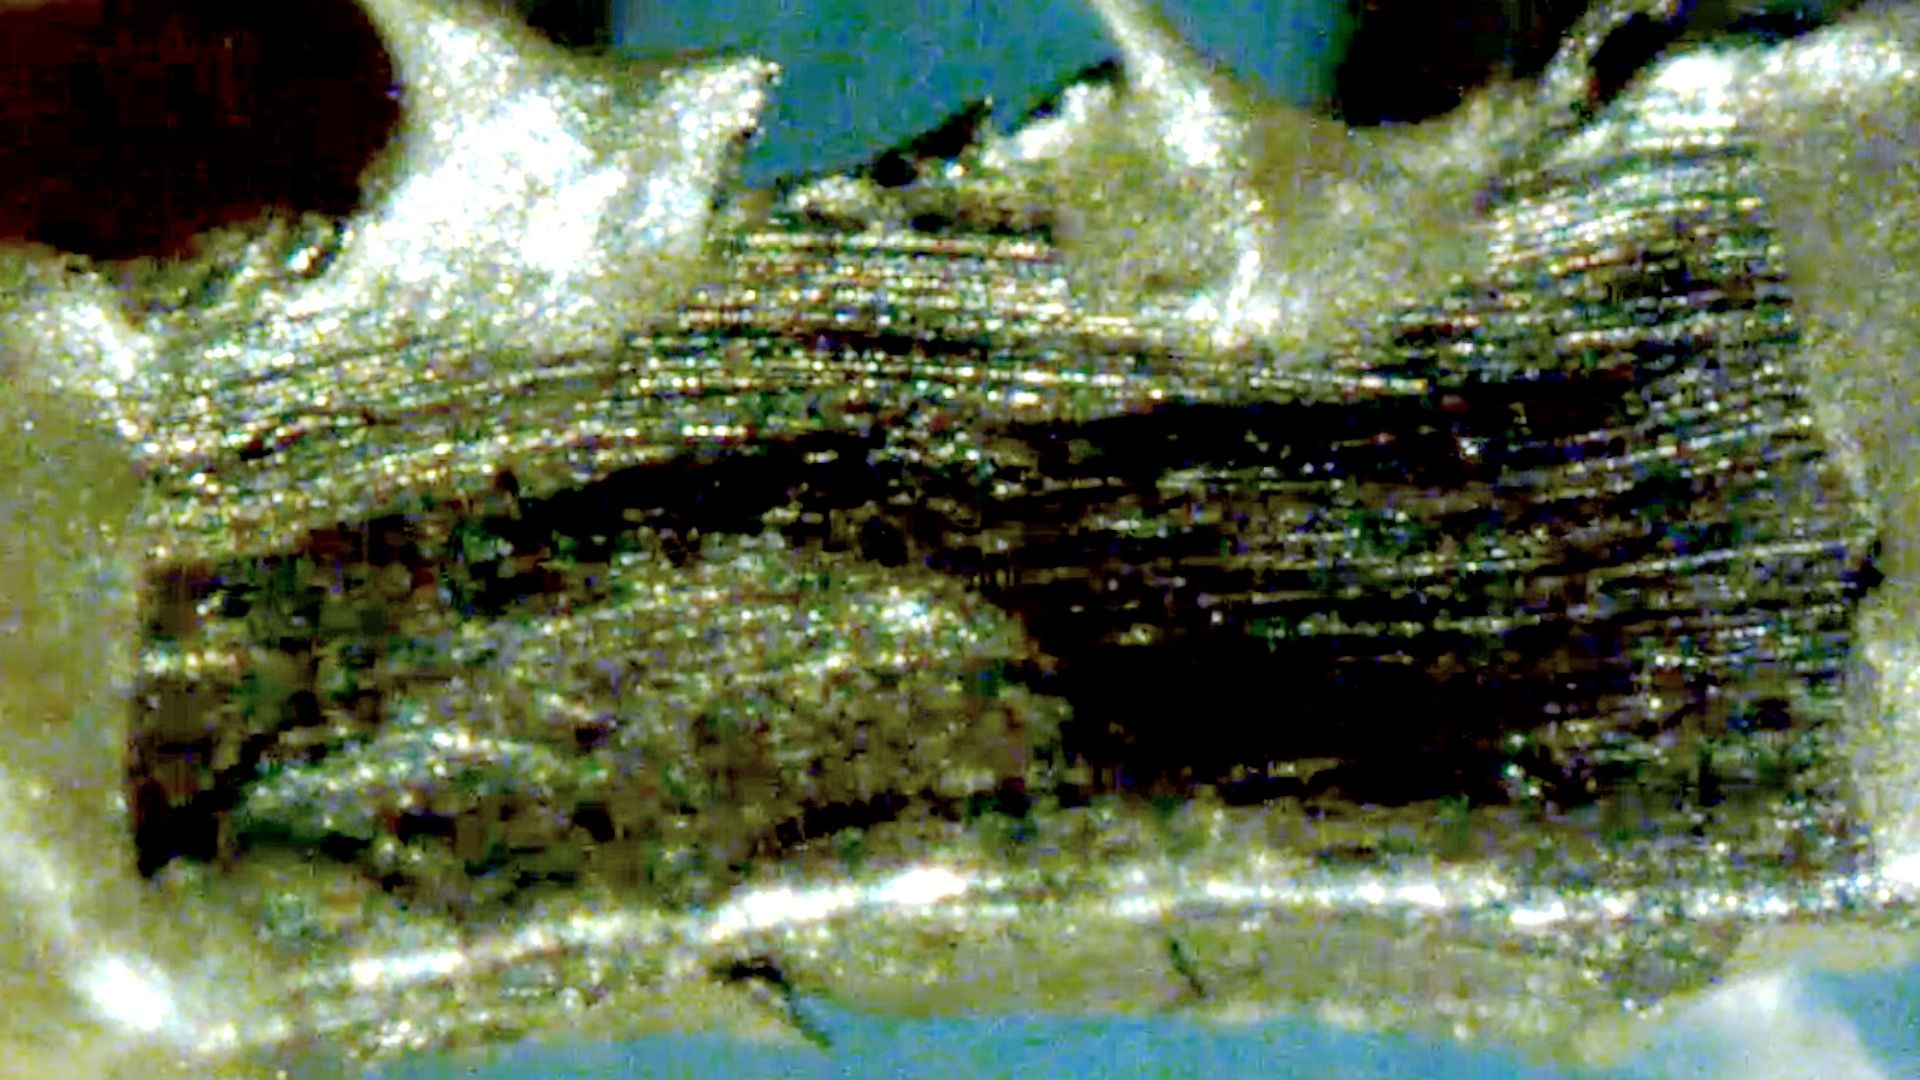
\includegraphics[width=\hsize]{results_discussions/190112_after_pulse17.eps}
  \end{center}
  \caption{}
  \label{fig:two}
 \end{minipage}
  \begin{minipage}{0.5\hsize}
  \begin{center}
   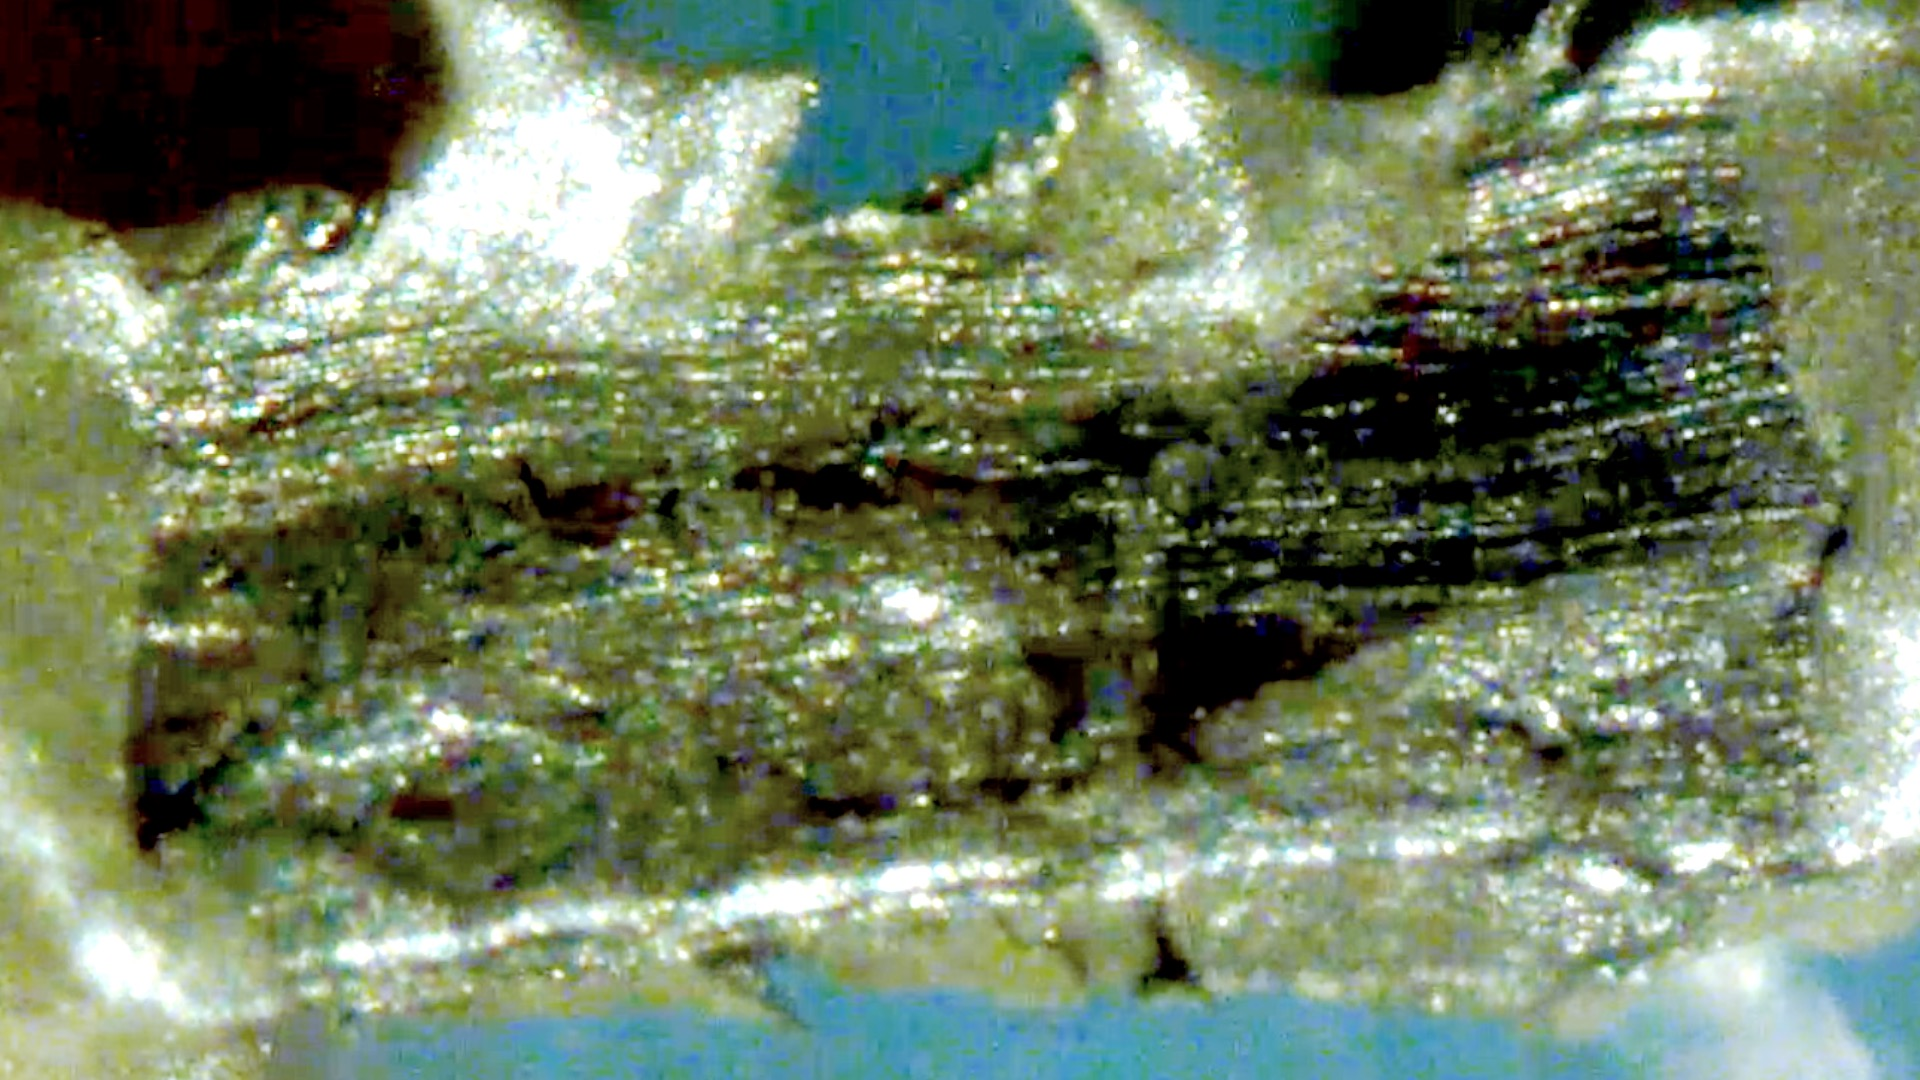
\includegraphics[width=\hsize]{results_discussions/190112_after_pulse19_1.eps}
  \end{center}
  \caption{}
  \label{fig:two}
 \end{minipage}
  \begin{minipage}{0.5\hsize}
  \begin{center}
   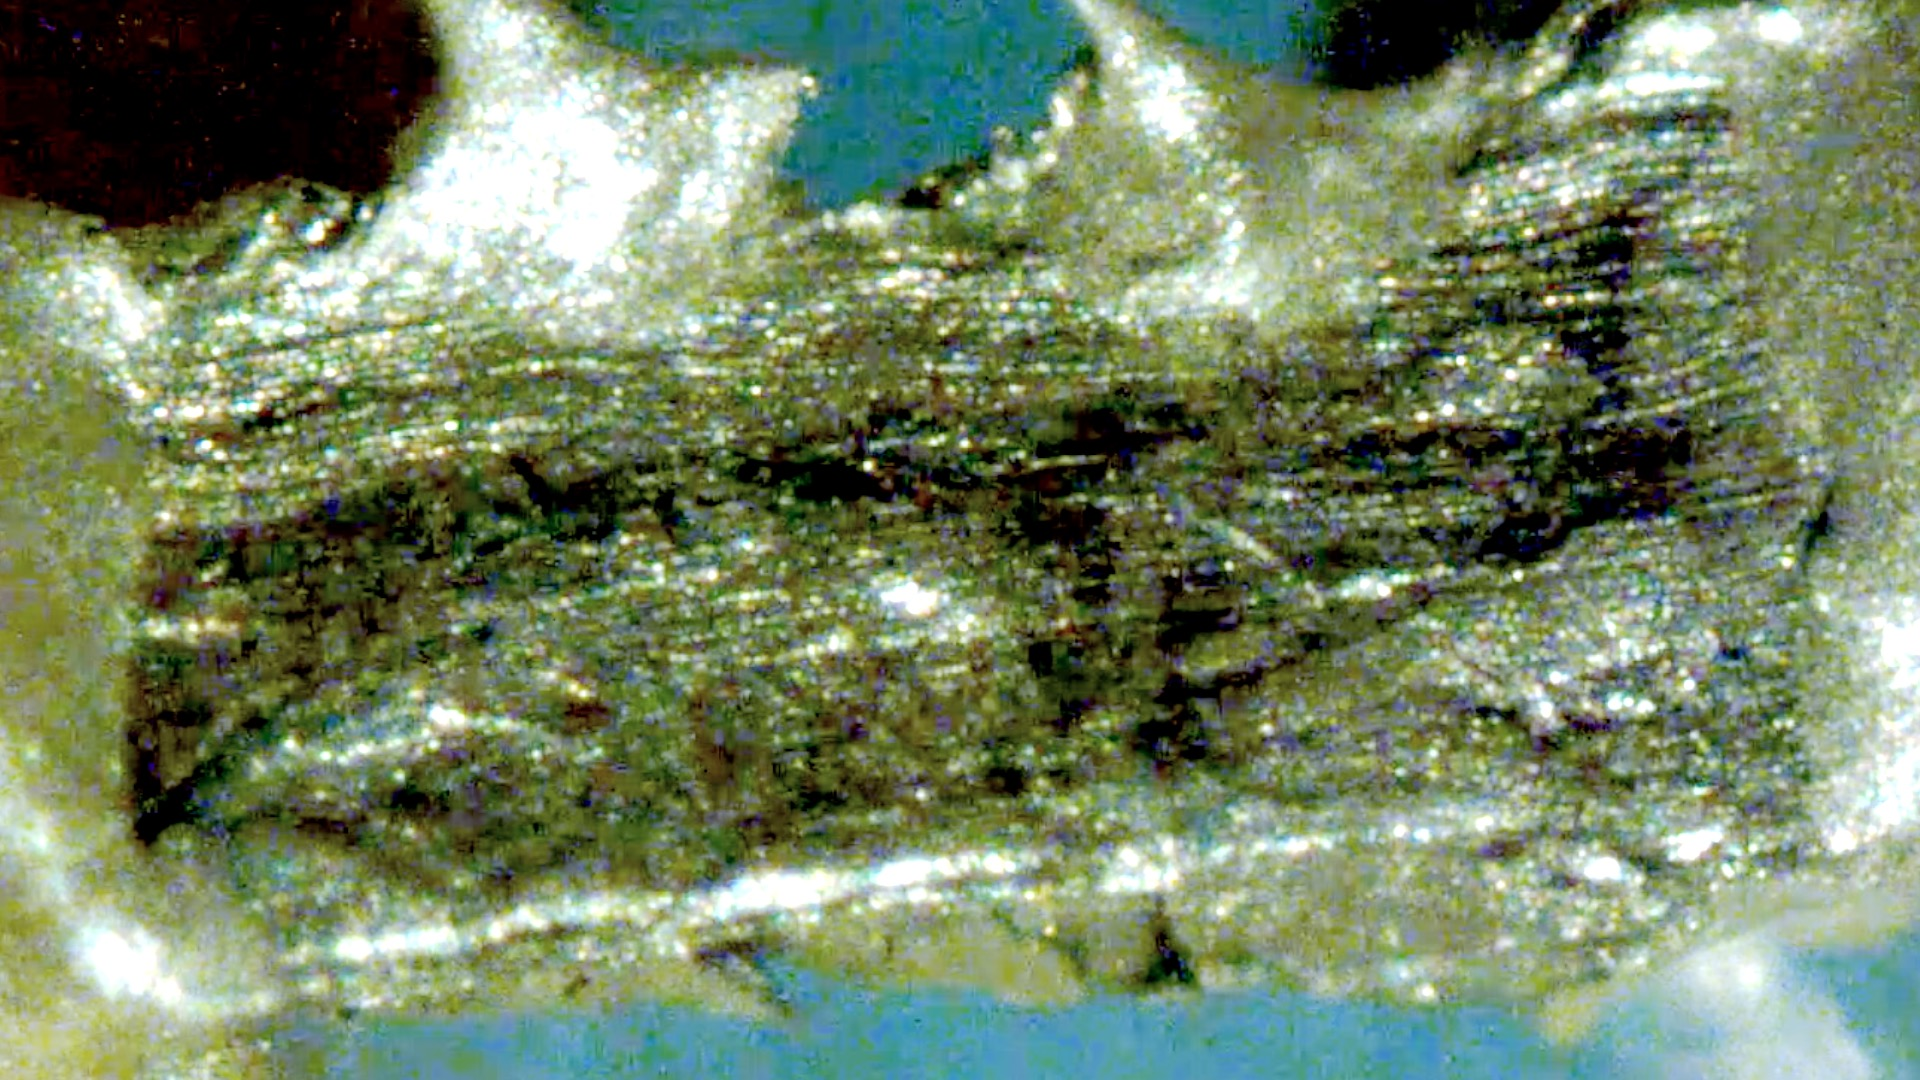
\includegraphics[width=\hsize]{results_discussions/190112_after_pulse19_2.eps}
  \end{center}
  \caption{}
  \label{fig:two}
 \end{minipage}
  \begin{minipage}{0.5\hsize}
  \begin{center}
   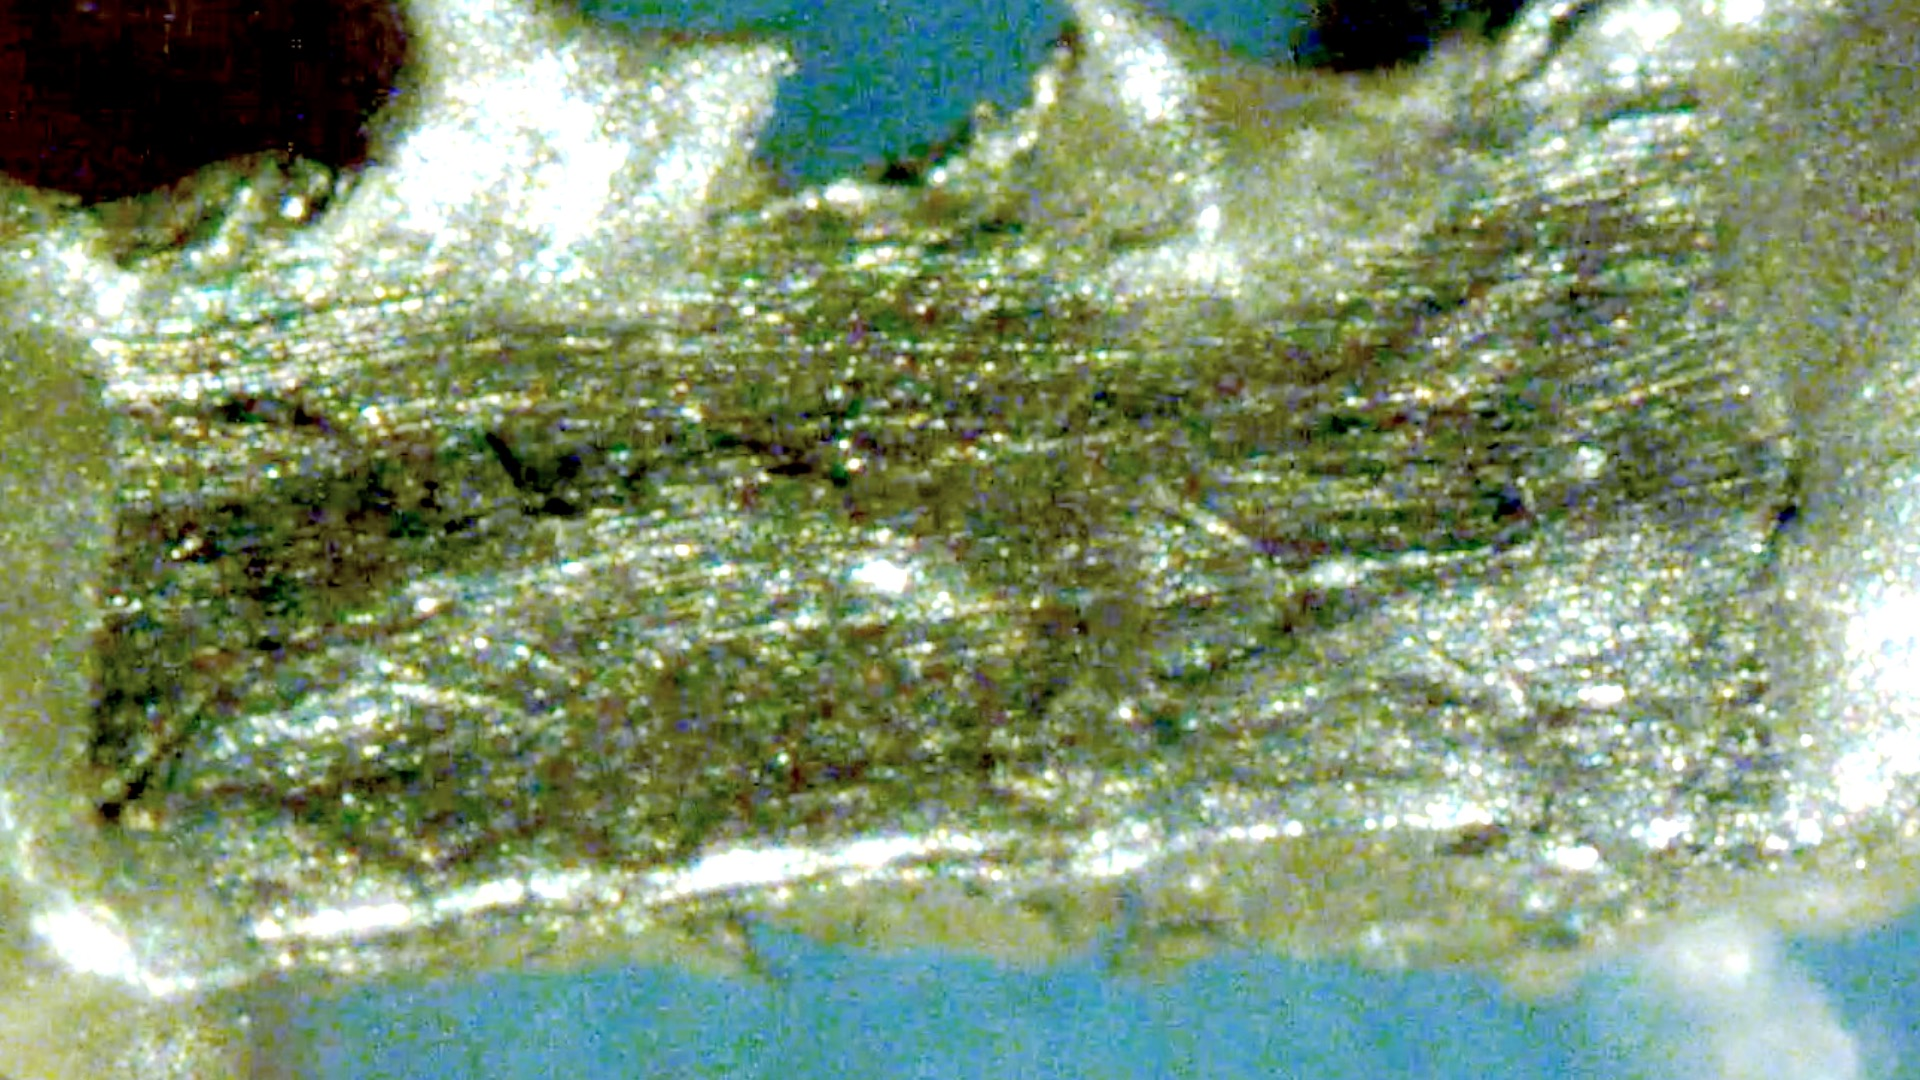
\includegraphics[width=\hsize]{results_discussions/190112_after_pulse20.eps}
  \end{center}
  \caption{}
  \label{fig:two}
 \end{minipage}
\end{figure}

\subsection{電流パルスを用いたβ相からα相への変換}

\newpage

%cd Documents/GitManagedProjects-Kagawalab/報告書/卒業論文/results_discussions/